\documentclass[10pt,twocolumn,letterpaper]{article}

\usepackage{cvpr}
\usepackage{times}
\usepackage{epsfig}
\usepackage{graphicx}
\usepackage{amsmath}
\usepackage{amssymb}
\usepackage{mathrsfs}

% Include other packages here, before hyperref.

% If you comment hyperref and then uncomment it, you should delete
% egpaper.aux before re-running latex.  (Or just hit 'q' on the first latex
% run, let it finish, and you should be clear).
\usepackage[breaklinks=true,bookmarks=false]{hyperref}

\graphicspath{ {./images/} }

\cvprfinalcopy % *** Uncomment this line for the final submission

\def\cvprPaperID{6969} % *** Enter the CVPR Paper ID here
\def\httilde{\mbox{\tt\raisebox{-.5ex}{\symbol{126}}}}

% Pages are numbered in submission mode, and unnumbered in camera-ready
%\ifcvprfinal\pagestyle{empty}\fi
\setcounter{page}{1}
\begin{document}

%%%%%%%%% TITLE
% \title{Final Project Proposal - <Copy paste from Ravi>}
\title{Implementing Learning-Based Light Field View Synthesis}

\author{Thomas Lauer\\
UC San Diego\\
9500 Gilman Drive, San Diego CA\\
{\tt\small tlauer@ucsd.edu}
% For a paper whose authors are all at the same institution,
% omit the following lines up until the closing ``}''.
% Additional authors and addresses can be added with ``\and'',
% just like the second author.
% To save space, use either the email address or home page, not both
\and
Winston Durand\\
UC San Diego\\
9500 Gilman Drive, San Diego CA\\
{\tt\small wdurand@ucsd.edu}
}

\maketitle
%\thispagestyle{empty}

%%%%%%%%% ABSTRACT
\begin{abstract}
Light field photography allows for the capture of images from multiple
perspectives using a single camera array or array of microlenses. However
these come at a tradeoff between spatial resolution and angular resolution.
As the number of the microlens elements increases, the resulting lightfields
have higher angular resolution which is useful for depth estimation,
but will have lower spatial resolution for novel view synthesis.
We implement the a paper on learning based method to synthesize views from light
field camera data \cite{LearningViewSynthesis} in PyTorch.
\end{abstract}

% GUIDELINES for proposal:
% a list of four to six milestones, and deadlines to achieve the milestones
% a list of questions to be answered during the project and discussed in the report
% if the project is experimental, which existing software you will use directly or build upon
% if the project is experimental, precisely which datasets you will use and where you can obtain them quickly
% a few recent and very closely related papers that you will build on, with full bibliographic data.

%%%%%%%%% BODY TEXT
\section{Introduction}

A Lytro is a common light field camera which uses microlenses to capture multiple
perspectives of a scene in one light field. 

% Insert summary of levoy 96 (this bit is related) (needs proper citation)
Kalantari summarizes several existing methods for interpolating lightfields and their drawbacks.
Many rely on high quality input images and well defined orientations between views,
which are difficult to achieve with consumer light field cameras, and impossible with light fields
captured by hand with cellphone cameras.

Many geometric methods novel view synthesis 
such as Levoy \etal~\cite{levoy1996light} require relatively high sample counts to ensure full
coverage of the 4D lightfield, as the simple linear interpolation used by Levoy
do not work well if there are heavily occluded regions or missing data.

Wanner \etal~\cite{Wanner} utilizes an optimization based approach, which calculates disparities
using traditional computer vision as a preprocessing step. However, because the disparity estimation
is independent from the loss function, it can not be optimized as part of the training process. 

Kalantari \etal~\cite{LearningViewSynthesis} propose a method to interpolate between 
sparsely sampled sub-apertures views. They use an $8 \times 8$ subset of the full $14 \times 14$ subaperture, since the
edge pixels are often black. The four corner sub-aperture views are fed into a series of two 
networks, the first is used to predict disparity which is then used to warp the sample images to the final perspective.
The second network then takes these warped images, along with some additional metadata, and blends them together
to produce the final RGB image of the novel view. Keeping this process differentiable allows both CNNs to 
be trained at the same time, which lets the disparity estimator become tuned to work with the final CNN.

\subsection{Our Proposal}

Our goal is to reimplement the paper \textit{Learning-Based View Synthesis for Light Field Cameras} by 
Kalantari \etal~\cite{LearningViewSynthesis} and additionally try to apply this technique to non-Lytro camera
array captures. Further, we would like to investigate rendering novel views outside of the planar
quadrilateral formed by the source images. To evaluate the performance of our model, we will use 
the structural similarity index measure (SSIM) and peak signal to noise ratio (PSNR), which are the 
same metrics used by the original paper.

\section{Technology}

We implemented this using PyTorch, because it has high performance, 
automatically handles calculating derivatives, and we have previous experience with it.
In addition, we used NumPy to compute the preprocessing and feature extraction of the input lightfields,
and SciPy for the image quality metrics.

We are not expecting to get real time performance, the paper claims it took 12.3 seconds to synthesize
a single image using a Matlab implementation. We will stitch the individual images into a video to
help visualize the results.

\section{Datasets}

We train our model using using Lytro captures since they represent a regularized input format with
online datasets easily available. In this paper, we make use of the Standford Lytro dataset by Raj \etal~\cite{StanfordLytro}
In addition to the ease of availability, these datasets also provide a 

\section{Implementation Details}

Our implementation closely follows that of Kalantari \etal~\cite{LearningViewSynthesis} with several modifications such
as being based on PyTorch \cite{PyTorch}.

\subsection{Preprocessing}

Each lightfield is cropped to only use the inner $8 \times 8$ grid of images out of the total $14 \times 14$ available
since the microlens actually captures a circle of data. For training, we additionally ignore the outer 60 pixels where
undesirable artifacts sometimes occur and train on $60\times60$ patches with a stride of 24 pixels to ensure overlap.
Each patch has its depth data estimated for all 64 ground truths and is saved to disk. Across the 68 images from the
Stanford Lytro dataset by Raj \etal~\cite{StanfordLytro}, we synthesize roughly 600,000 unique patch views total split
90/10 between training and validation passes.

\subsection{Network}

Our network was implemented using PyTorch, using two separate convolutional networks to perform the
disparity estimation and final color assembly. Our disparity estimation network takes a 
$200 \times H \times W$ tensor as input, which we calculate using the preprocessing step.

Here is the architecture of the disparity estimation network.

\begin{center}
\begin{tabular}{|c c c c|}
    Input & Output & Kernel Size & Activation \\
    \hline
    200 & 100 & $7 \times 7$ & ReLU \\
    100 & 100 & $5 \times 5$ & ReLU \\
    100 & 50 & $3 \times 3$ & ReLU \\
    50 & 1 & $1 \times 1$ & None \\
\end{tabular}
\end{center}


This disparity is then used to warp the 4 input views using the following equation:

$$
\overline{L}_{p_i} = L_{p_i} \left[ s + \left(p_i - q\right) D_q(s) \right]
$$

Where $s$ is the pixel location, $p_i$ is the location of the input view, and $q$ is the location of the
desired novel view. $D_q(s)$ is the estimated disparity at the pixel from the depth estimation network,
and $L_{p_i}(s)$ is the color of the novel view. We use the grid\_sample function from PyTorch, which integrates
with autograd to allow backpropegating the weights through $L_{p_i}(s)$. $s$, $p_i$, and $q$ are all 
constant precalculated inputs, but autograd is able to compute the derivative 
$\frac{\partial \overline{L}_{p_i}}{\partial D_q}$ automatically. 

These four RGB images, along with the $u$ and $v$ 
locations of the desired novel view and the disparity estimate from the first network are concatonated
together into a single 15 channel image. Kalantari \etal name this image $H$. This is used as the input to the color estimation network, which
has the following architecture:

\begin{center}
\begin{tabular}{|c c c c|}
    Input & Output & Kernel Size & Activation \\
    \hline
    15 & 100 & $7 \times 7$ & ReLU \\
    100 & 100 & $5 \times 5$ & ReLU \\
    100 & 50 & $3 \times 3$ & ReLU \\
    50 & 3 & $1 \times 1$ & None \\
\end{tabular}
\end{center}

Because none of the convolutions have padding, the network loses 12 pixels on each edge, reducing
the $60 \times 60$ patches during training to $36 \times 36$. Training without padding is ideal in this situation, 
because it would make the training patches less representative of the entire image.

\subsection{Training}

Our loss function is directly the $\mathcal{L}_2$ distance between the channel wise RGB values of the novel image
and the ground truth image. While Kalantari \etal needed to numerically calculate the gradient of the interpolation
step which warps the ground truth images to the novel viewpoint, PyTorch's autograd is able to handle this automatically.
We needed to be careful to not destroy the gradient chain while calculating $s + \left(p_i - q\right) D_q(s)$, which had
to be done manually outside of a PyTorch function, because of the way autograd builds the sequence of operations to backpropegate on.

We used the ADAM optimizer with a learning rate of $1e-3$, $\beta_1 = 0.9$, $\beta_2 = 0.999$, and $eps = 1e-8$. Our batch size 
is 64 $60 \times 60$ patches. Our training loop runs on 8951 batches, which gives a total of 553,664 patches and over 700 million
individual pixels to train on. This is significantly more data than the roughly 100,000 patches Kalanatri \etal trained on.
Our implementation is also significantly faster than theirs, it took their network 12.3 seconds to generate a novel viewpoint
whereas ours takes 6.2 seconds. We believe this is mostly because of improvements in hardware from 2016, and has little to do with the
actual algorithms.

\section{Results}

Because of the much larger datset, we have currently trained for 17 epochs. We are currently training up to 100 epochs, but we 
wanted to be sure we had some metrics for this preliminary report. For this reason, we expect that our results will perform worse
than our final versions. 

These are the structural similarity scores and peak signal to noise ratio scores of our images compared to the ground truth.

\pagebreak

\begin{center}
Flowers and Plants 25

\begin{tabular}{|c c c|}
    Network & SSIM & PSNR \\ \hline
    Ours & 0.898 & 31.48 \\
    Reference & 0.931 & 33.19 \\ 
\end{tabular}
\end{center}

\medspace

\begin{center}
Rocks

\begin{tabular}{|c c c|}
    Network & SSIM & PSNR \\ \hline
    Ours & 0.841 & 26.41 \\
    Reference & 0.969 & 34.66 \\ 
    Wanner and Goldluecke & 0.488 & 16.57 
\end{tabular}
\end{center}


Here is an example from the Stanford Light Field Archive, specifically Flowers and Plants number 25.
The different crop factors are because Kalantari \etal decided to 

\begin{figure}[h]
\begin{center}
\caption{Kalantari \etal Flowers 25}
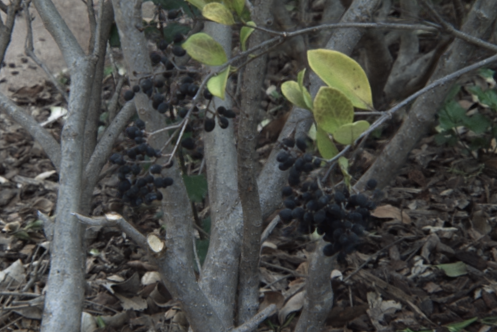
\includegraphics[width=8cm]{flowers_25/kalantari_05_05.png}
\end{center}
\end{figure}

\begin{figure}[h]
\begin{center}
\caption{Our Flowers 25}
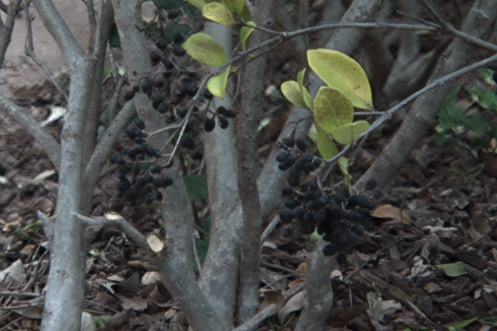
\includegraphics[width=8cm]{flowers_25/ours_05_05.png}
\end{center}
\end{figure}

\begin{figure}[h]
\begin{center}
\caption{Ground Truth Flowers 25}
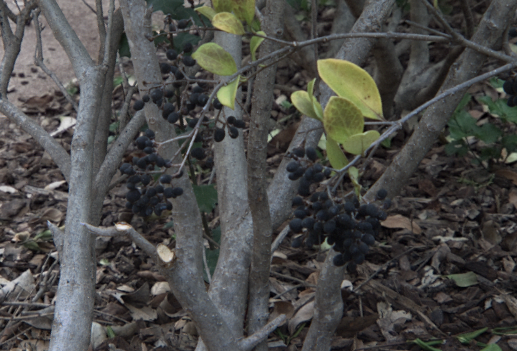
\includegraphics[width=8cm]{flowers_25/truth_05_05.png}
\end{center}
\end{figure}


Here are the results from the rock example Kalantari uses. We used a subset of the Stanford Lytro Archive to train, and are
going to retrain the network using their light fields that they captured. Our network does need a lot more training time
at this point, but still performs well compared to other implementations such as Wanner and Goldluecke, even though
it is seriously under trained. 

\begin{figure}[h]
\begin{center}
\caption{Kalantari \etal Rock}
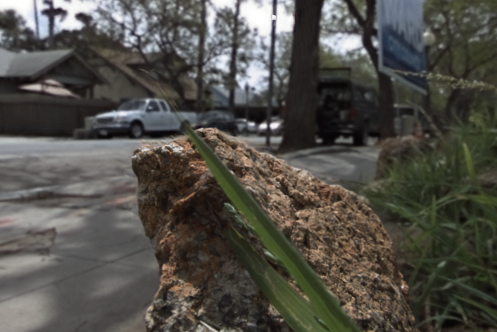
\includegraphics[width=8cm]{rock/kalantari_05_05.png}
\end{center}
\end{figure}

\begin{figure}[h]
\begin{center}
\caption{Our Rock}
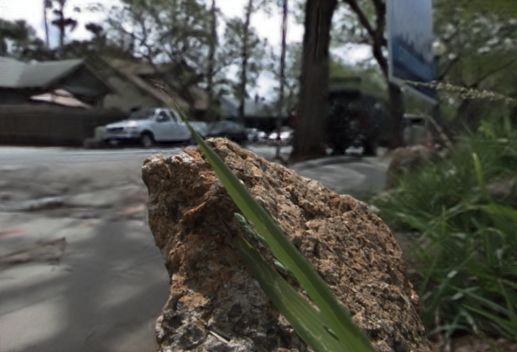
\includegraphics[width=8cm]{rock/ours_05_05.png}
\end{center}
\end{figure}

\begin{figure}[h]
\begin{center}
\caption{Ground Truth Rock}
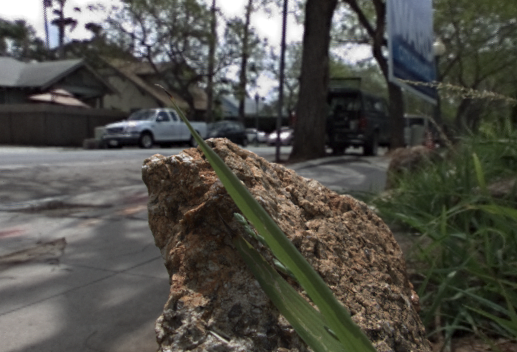
\includegraphics[width=8cm]{rock/truth_05_05.png}
\end{center}
\end{figure}


\pagebreak

{\small
\bibliographystyle{ieee_fullname}
\bibliography{egbib}
}

\end{document}
